% Báo cáo BTL Vật lý 1 - Bài 6. Biên dịch bằng XeLaTeX:
%   latexmk -xelatex main.tex
\documentclass[13pt,a4paper,oneside]{extreport}
\usepackage{fontspec}
\setmainfont{TeX Gyre Termes}          % Times; đổi thành Times New Roman nếu máy có
\usepackage[left=3cm,right=2cm,top=2.5cm,bottom=2.5cm]{geometry}
\usepackage{amsmath,amssymb,siunitx}
\usepackage{graphicx,float,caption,booktabs,array,longtable}
\usepackage{setspace}\onehalfspacing
\usepackage{titlesec,tocloft}
\usepackage{listings,xcolor}
\usepackage[hidelinks]{hyperref}
\usepackage{indentfirst}
\usepackage{enumitem}

\graphicspath{{../figures/}}
\sisetup{output-decimal-marker={,}}

% Tiêu đề chương: "CHƯƠNG 1. TÊN CHƯƠNG" theo mẫu
\titleformat{\chapter}[hang]{\normalfont\large\bfseries\centering}{CHƯƠNG \thechapter.}{0.5em}{}
\titlespacing*{\chapter}{0pt}{0pt}{18pt}
\titleformat{\section}{\normalfont\bfseries}{\thesection.}{0.5em}{}
\titleformat{\subsection}{\normalfont\bfseries\itshape}{\thesubsection.}{0.5em}{}
% Tiêu đề Mục lục / Danh sách hình / bảng: căn giữa, cỡ như tiêu đề chương
\renewcommand{\cfttoctitlefont}{\hfill\large\bfseries}\renewcommand{\cftaftertoctitle}{\hfill}
\renewcommand{\cftloftitlefont}{\hfill\large\bfseries}\renewcommand{\cftafterloftitle}{\hfill}
\renewcommand{\cftlottitlefont}{\hfill\large\bfseries}\renewcommand{\cftafterlottitle}{\hfill}
\setlength{\cftbeforetoctitleskip}{0pt}\setlength{\cftbeforeloftitleskip}{0pt}\setlength{\cftbeforelottitleskip}{0pt}
\titleformat{name=\chapter,numberless}[hang]{\normalfont\large\bfseries\centering}{}{0pt}{}
\titlespacing*{name=\chapter,numberless}{0pt}{0pt}{18pt}
\renewcommand{\cftchapfont}{\bfseries}
\renewcommand{\cftchappresnum}{CHƯƠNG }
\renewcommand{\cftchapaftersnum}{.}
\setlength{\cftchapnumwidth}{6em}
\renewcommand{\cftsecaftersnum}{.}
\renewcommand{\cftdotsep}{2}
\renewcommand{\cftchapleader}{\cftdotfill{\cftdotsep}}

% Tên mục bằng tiếng Việt
  \renewcommand{\contentsname}{MỤC LỤC}%
  \renewcommand{\listfigurename}{DANH SÁCH HÌNH VẼ}%
  \renewcommand{\listtablename}{DANH SÁCH BẢNG}%
  \renewcommand{\bibname}{TÀI LIỆU THAM KHẢO}%
  \renewcommand{\figurename}{Hình}%
  \renewcommand{\tablename}{Bảng}%
  \renewcommand{\appendixname}{Phụ lục}

% Mã nguồn MATLAB trong phụ lục
\lstset{language=Matlab, basicstyle=\ttfamily\small, breaklines=true,
  numbers=left, numberstyle=\tiny, frame=single, extendedchars=true,
  inputencoding=utf8, keywordstyle=\color{blue}, commentstyle=\color{green!50!black},
  stringstyle=\color{purple}, showstringspaces=false}

% Chương không đánh số nhưng có trong mục lục
\newcommand{\unnumberedchapter}[1]{\chapter*{#1}\addcontentsline{toc}{chapter}{#1}}

\begin{document}
\begin{titlepage}
\begin{center}
{\large ĐẠI HỌC QUỐC GIA TP. HỒ CHÍ MINH}\\
{\large\bfseries TRƯỜNG ĐẠI HỌC BÁCH KHOA}\\
{\large\bfseries KHOA KHOA HỌC ỨNG DỤNG}\\[1.5cm]
% 
\includegraphics[width=4cm]{logo_hcmut}\\[1.5cm]  % thêm logo nếu có
\vspace{2cm}
{\LARGE\bfseries BÁO CÁO BÀI TẬP LỚN}\\[0.4cm]
{\Large\bfseries MÔN HỌC: VẬT LÝ 1}\\[1.5cm]
{\large\bfseries ĐỀ TÀI (BÀI 6):}\\[0.3cm]
{\large\bfseries VẼ QUỸ ĐẠO CHUYỂN ĐỘNG NÉM XIÊN TRONG TRỌNG TRƯỜNG BỎ QUA LỰC CẢN VÀ XÁC ĐỊNH MỘT SỐ THÔNG SỐ LIÊN QUAN}\\[2cm]
{\bfseries LỚP: L06 --- NHÓM: 5}\\[0.3cm]
{\bfseries GIẢNG VIÊN HƯỚNG DẪN: CÔ NGUYỄN LÊ BẢO THƯ}
\vfill
{\bfseries TP. HỒ CHÍ MINH, THÁNG 11/2026}
\end{center}
\end{titlepage}

% Bìa phụ (theo mẫu): không khung, danh sách thành viên kèm MSSV
\begin{titlepage}
\newgeometry{left=2.5cm,right=2.5cm,top=2cm,bottom=2cm}
\centering\setstretch{1}
{\fs{16}\bfseries ĐẠI HỌC QUỐC GIA TP. HỒ CHÍ MINH\\
TRƯỜNG ĐẠI HỌC BÁCH KHOA\\
KHOA KHOA HỌC ỨNG DỤNG\par}
\vspace{0.6cm}

\includegraphics[width=2cm]{logo_hcmut}\par
\vspace{0.5cm}
{\fs{18}\bfseries BÁO CÁO BÀI TẬP LỚN\par}
\vspace{1.6cm}
{\fs{20}\bfseries VẼ QUỸ ĐẠO CHUYỂN ĐỘNG NÉM XIÊN TRONG TRỌNG TRƯỜNG BỎ QUA LỰC CẢN VÀ XÁC ĐỊNH MỘT SỐ THÔNG SỐ LIÊN QUAN\par}
\vspace{3.4cm}
{\fs{16}\bfseries
\begin{tabular}{@{}l@{\hspace{0.6cm}}l@{\hspace{0.8cm}}l@{}}
\multicolumn{3}{@{}l}{Nhóm 5 -- Lớp L06:}\\[4pt]
1.  & Nguyễn Bảo Vy          & {\fs{13}MSSV: 2612906} \\
2.  & Nguyễn Cao Gia Bảo     & {\fs{13}MSSV: 2612707} \\
3.  & Nguyễn Cao Trọng Trung & {\fs{13}MSSV: 2610226} \\
4.  & Nguyễn Công Hiếu       & {\fs{13}MSSV: 2613497} \\
5.  & Nguyễn Đăng Khôi       & {\fs{13}MSSV: 2610289} \\
6.  & Nguyễn Đình Bảo        & {\fs{13}MSSV: 2612708} \\
7.  & Nguyễn Dương Minh Hiếu & {\fs{13}MSSV: 2613627} \\
8.  & Nguyễn Duy Quang       & {\fs{13}MSSV: 2613666} \\
9.  & Nguyễn Gia Lộc         & {\fs{13}MSSV: 2613342} \\
10. & Nguyễn Hòa Anh Chương  & {\fs{13}MSSV: 2210396} \\
\end{tabular}\par}
\vfill
{\fs{14}\bfseries Tp. HCM, 11/2026\par}
\restoregeometry
\end{titlepage}


\pagenumbering{roman}
\unnumberedchapter{TÓM TẮT BÀI BÁO CÁO}  % TODO: dán nội dung từ Google Docs vào đây.

\unnumberedchapter{LỜI CẢM ƠN}           % TODO: dán nội dung từ Google Docs vào đây.

\clearpage\tableofcontents
\clearpage\addcontentsline{toc}{chapter}{DANH SÁCH HÌNH VẼ}\listoffigures
\clearpage\addcontentsline{toc}{chapter}{DANH SÁCH BẢNG}\listoftables
\unnumberedchapter{DANH MỤC CÁC TỪ VIẾT TẮT} \begin{tabular}{ll}
BTL & Bài tập lớn \\
% TODO: bổ sung các từ viết tắt khác
\end{tabular}

\unnumberedchapter{YÊU CẦU ĐỀ TÀI ĐƯỢC GIAO} % TODO: dán nội dung từ Google Docs vào đây. (TV1 -- Công Hiếu)


\clearpage\pagenumbering{arabic}
% Chương 1 - Nguồn: TV2 (Đình Bảo), Google Doc "Workspace Nhóm - BTL Vật Lý 1 2026"
\chapter{CƠ SỞ LÝ THUYẾT VẬT LÝ VỀ CHUYỂN ĐỘNG NÉM XIÊN}\label{chap:lythuyet}

\section{Các giả thiết lý tưởng và thiết lập hệ trục tọa độ Oxy}

\subsection{Định nghĩa}
Ném xiên là chuyển động của một vật được ném lên với một vận tốc ban đầu hợp với phương ngang một góc $\alpha$ và vật chỉ chịu tác dụng của trọng lực.

\subsection{Các giả thiết}
\begin{itemize}
  \item Bỏ qua mọi lực cản của không khí tác dụng lên vật.
  \item Xem vật là chất điểm.
  \item Gia tốc trọng trường $\vec{g}$ là hằng số, không đổi cả về hướng lẫn độ lớn, do độ cao bay và tầm xa rất nhỏ so với bán kính Trái Đất.
  \item Mặt đất được coi là mặt phẳng ngang; hệ quy chiếu gắn với mặt đất được coi là hệ quy chiếu quán tính (bỏ qua sự tự quay của Trái Đất, do đó bỏ qua lực quán tính Coriolis).
\end{itemize}

\subsection{Ký hiệu và đơn vị}
Các đại lượng đã cho:
\begin{itemize}
  \item Vận tốc ban đầu $v_0$: tốc độ tại thời điểm vật bắt đầu được ném, $v_0 > 0$ (m/s).
  \item Góc ném $\alpha$: góc hợp bởi vectơ vận tốc ban đầu và phương ngang Ox, với $0^\circ < \alpha < 90^\circ$ (đơn vị: độ hoặc rad).
  \item Gia tốc trọng trường $g$: gia tốc do lực hút Trái Đất gây ra, luôn hướng thẳng đứng xuống dưới (lấy bằng $9{,}81~\mathrm{m/s^2}$).
\end{itemize}
Các đại lượng cần xác định:
\begin{itemize}
  \item $R$: tầm ném xa (m).
  \item $H$: độ cao cực đại (m).
  \item $T$: thời gian bay (s).
\end{itemize}

\subsection{Hệ tọa độ Oxy}
\begin{itemize}
  \item Gốc tọa độ O: đặt tại vị trí ném vật ở thời điểm ban đầu $t = 0$.
  \item Trục Ox: nằm ngang, hướng theo chiều hình chiếu ngang của vận tốc ban đầu.
  \item Trục Oy: thẳng đứng, hướng lên trên (xem Hình~\ref{fig:nemxien}).
\end{itemize}

\begin{figure}[H]
  \centering
  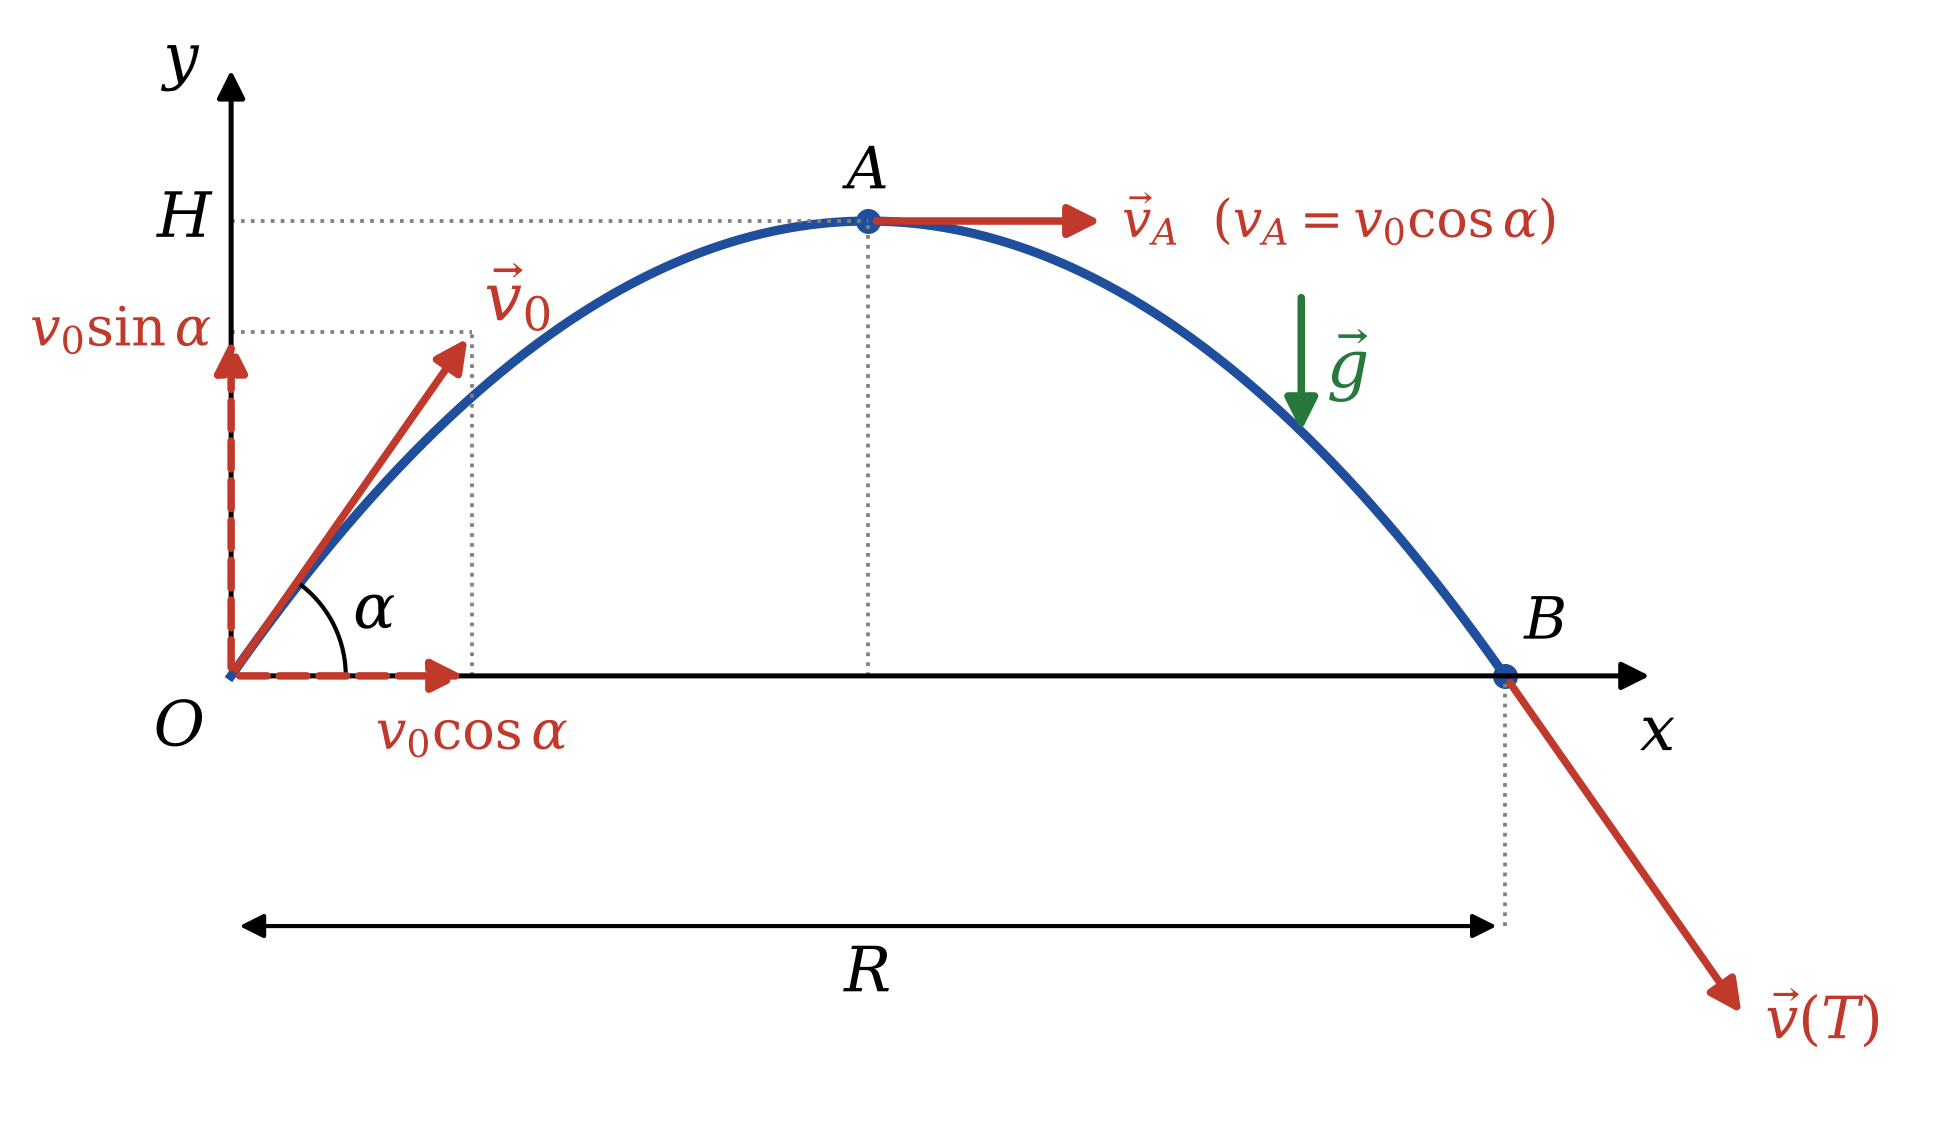
\includegraphics[width=0.85\textwidth]{hinh1_1_nemxien.png}
  \caption{Quỹ đạo chuyển động ném xiên và các đại lượng đặc trưng trong hệ tọa độ Oxy}
  \label{fig:nemxien}
\end{figure}

\section{Phương trình vi phân chuyển động và quy luật động học}
Theo định luật II Newton, phương trình vectơ chuyển động của vật chỉ chịu tác dụng của trọng lực $\vec{P} = m\vec{g}$ là:
\[ m\vec{a} = \vec{P} = m\vec{g} \]
Suy ra:
\[ \vec{a} = \vec{g} \]
Như vậy, gia tốc của vật bằng gia tốc trọng trường $\vec{g}$ và không phụ thuộc vào khối lượng $m$ của vật. Chiếu phương trình vectơ này lên hai trục tọa độ, ta thu được các phương trình sau.

Phương trình vi phân:
\begin{itemize}
  \item Trục Ox: $a_x = \dfrac{\mathrm{d}^2x}{\mathrm{d}t^2} = 0$: chuyển động hình chiếu trên trục Ox là chuyển động thẳng đều.
  \item Trục Oy: $a_y = \dfrac{\mathrm{d}^2y}{\mathrm{d}t^2} = -g$: chuyển động hình chiếu trên trục Oy là chuyển động thẳng biến đổi đều. Dấu ``$-$'' xuất hiện vì $\vec{g}$ ngược chiều trục Oy ($g > 0$ là độ lớn gia tốc trọng trường).
\end{itemize}

Tại thời điểm ban đầu $t = 0$, vật được ném từ gốc tọa độ với vận tốc ban đầu $v_0$ hợp với phương ngang góc $\alpha$:
\begin{itemize}
  \item Tọa độ ban đầu: $x(0) = 0$, \ $y(0) = 0$.
  \item Vận tốc ban đầu: $v_x(0) = v_0\cos\alpha$, \ $v_y(0) = v_0\sin\alpha$.
\end{itemize}

Vận tốc theo thời gian: lấy tích phân hai vế phương trình vi phân gia tốc theo thời gian $t$, sau đó thay vận tốc ban đầu, ta được phương trình vận tốc:
\begin{align*}
  v_x(t) &= \int 0\,\mathrm{d}t = C_1,
    & \text{tại } t = 0:\ v_x(0) &= v_0\cos\alpha \;\Rightarrow\; C_1 = v_0\cos\alpha \\
  v_y(t) &= \int (-g)\,\mathrm{d}t = -gt + C_2,
    & \text{tại } t = 0:\ v_y(0) &= v_0\sin\alpha \;\Rightarrow\; C_2 = v_0\sin\alpha
\end{align*}
Suy ra:
\[ v_x(t) = v_0\cos\alpha, \qquad v_y(t) = -gt + v_0\sin\alpha \]

Phương trình tọa độ: tiếp tục lấy tích phân hai vế phương trình vận tốc theo thời gian $t$, sau đó áp dụng điều kiện tọa độ ban đầu, ta được:
\[ x(t) = \int v_0\cos\alpha\,\mathrm{d}t = (v_0\cos\alpha)\,t + C_3; \qquad x(0) = 0 \Rightarrow C_3 = 0 \]
\begin{equation}
  x(t) = v_0\cos\alpha\cdot t
  \label{eq:x}
\end{equation}
\[ y(t) = \int (-gt + v_0\sin\alpha)\,\mathrm{d}t = -\frac{1}{2}gt^2 + (v_0\sin\alpha)\,t + C_4; \qquad y(0) = 0 \Rightarrow C_4 = 0 \]
\begin{equation}
  y(t) = -\frac{1}{2}gt^2 + v_0\sin\alpha\cdot t
  \label{eq:y}
\end{equation}

\section{Phương trình quỹ đạo chuyển động}
Để xác định phương trình quỹ đạo, trước tiên ta rút $t$ theo $x$ từ phương trình \eqref{eq:x}:
\[ t = \frac{x}{v_0\cos\alpha} \]
Thay biểu thức $t$ theo $x$ vào phương trình \eqref{eq:y}, ta được:
\[ y = \frac{v_0\sin\alpha\cdot x}{v_0\cos\alpha} - \frac{1}{2}g\left(\frac{x}{v_0\cos\alpha}\right)^2 \]
Rút gọn biểu thức trên, ta có:
\begin{equation}
  y = x\tan\alpha - \frac{g\,x^2}{2v_0^2\cos^2\alpha}
  \label{eq:quydao}
\end{equation}
Đây là phương trình bậc hai có dạng $y = ax^2 + bx + c$, trong đó:
\begin{itemize}
  \item $b = \tan\alpha$, \ $c = 0$;
  \item $a = -\dfrac{g}{2v_0^2\cos^2\alpha} < 0$.
\end{itemize}
Vì hệ số $a$ âm nên đạo hàm bậc hai của hàm số luôn âm. Do đó, quỹ đạo của chuyển động ném xiên là một đường parabol có bề lõm hướng xuống dưới. Phương trình \eqref{eq:quydao} chỉ áp dụng khi $\alpha \neq 90^\circ$ (vì khi rút $t$ theo $x$ đã chia cho $\cos\alpha$) và chỉ có nghĩa trong đoạn $0 \le x \le R$.

\section{Thiết lập công thức giải tích cho tầm xa \texorpdfstring{($R$)}{(R)}, độ cao cực đại \texorpdfstring{($H$)}{(H)} và thời gian bay \texorpdfstring{($T$)}{(T)}}
Các công thức dưới đây áp dụng khi vật được ném từ mặt đất và rơi trở lại cùng độ cao ban đầu.

\subsection{Thời gian bay \texorpdfstring{($T$)}{(T)}}
Vật chạm đất khi tọa độ theo phương thẳng đứng trở về giá trị ban đầu, tức là $y = 0$.

Thay $y = 0$ vào phương trình \eqref{eq:y}, sau đó phân tích thành nhân tử. Bỏ nghiệm $t = 0$ tương ứng với thời điểm bắt đầu ném, nghiệm còn lại là thời gian bay $T$:
\[ t\left(v_0\sin\alpha - \frac{gt}{2}\right) = 0 \;\Rightarrow\; t = 0 \ \text{hoặc}\ t = T \]
\begin{equation}
  T = \frac{2v_0\sin\alpha}{g}
  \label{eq:T}
\end{equation}

\subsection{Độ cao cực đại \texorpdfstring{($H$)}{(H)}}
Tại điểm cao nhất A của quỹ đạo (Hình~\ref{fig:nemxien}), vận tốc theo phương thẳng đứng bằng 0, tức là $v_y = 0$.

Từ phương trình vận tốc theo thời gian, suy ra thời điểm vật đạt độ cao cực đại:
\[ t_H = \frac{v_0\sin\alpha}{g} \]
So sánh với \eqref{eq:T}, ta có:
\[ t_H = \frac{T}{2} \]
Điều này cho thấy thời gian vật đi lên bằng thời gian vật đi xuống khi vật được ném và rơi trở lại cùng một độ cao.

Để xác định độ cao cực đại, thay $t_H = v_0\sin\alpha/g$ vào phương trình \eqref{eq:y}, quy đồng mẫu số và rút gọn, ta thu được công thức cuối cùng:
\begin{equation}
  H = v_0\sin\alpha\cdot t_H - \frac{g\,t_H^2}{2}
    = \frac{v_0^2\sin^2\alpha}{g} - \frac{v_0^2\sin^2\alpha}{2g}
    = \frac{v_0^2\sin^2\alpha}{2g}
  \label{eq:H}
\end{equation}

\subsection{Tầm xa \texorpdfstring{($R$)}{(R)}}
Tầm xa là khoảng cách theo phương ngang từ điểm ném O đến điểm rơi B của vật (Hình~\ref{fig:nemxien}). Khi vật chạm đất, $t = T$.

Thay $T = 2v_0\sin\alpha/g$ vào phương trình \eqref{eq:x}, rút gọn và sử dụng công thức lượng giác:
\[ \sin 2\alpha = 2\sin\alpha\cos\alpha \]
Suy ra công thức tính tầm xa:
\begin{equation}
  R = v_0\cos\alpha\cdot T = \frac{2v_0^2\sin\alpha\cos\alpha}{g} = \frac{v_0^2\sin 2\alpha}{g}
  \label{eq:R}
\end{equation}
Kiểm tra thứ nguyên: $[v_0^2/g] = (\mathrm{m^2/s^2})/(\mathrm{m/s^2}) = \mathrm{m}$, nên $R$ và $H$ có đơn vị mét; $[v_0/g] = (\mathrm{m/s})/(\mathrm{m/s^2}) = \mathrm{s}$, nên $T$ có đơn vị giây.

\subsection{Vận tốc lúc chạm đất}
Tại thời điểm chạm đất $t = T$:
\[ v_x(T) = v_0\cos\alpha; \qquad v_y(T) = v_0\sin\alpha - gT = -v_0\sin\alpha \]
Do đó độ lớn vận tốc lúc chạm đất bằng $v_0$; vectơ vận tốc hướng xuống và hợp với phương ngang góc $\alpha$. Kết quả này phù hợp với định luật bảo toàn cơ năng vì điểm ném và điểm rơi ở cùng độ cao.

% Chương 2 - Nguồn: TV3 (Vy), Google Doc "Workspace Nhóm - BTL Vật Lý 1 2026"
\chapter{PHÂN TÍCH TOÁN HỌC VÀ BIỆN LUẬN NGHIỆM GÓC NÉM}\label{chap:toanhoc}

\section{Đặt bài toán tìm góc ném thứ hai}
Trong chương trước, các phương trình chuyển động của vật ném xiên trong trọng trường đều (bỏ qua lực cản không khí) đã được thiết lập. Tầm xa của vật 1 ném lên từ mặt đất với vận tốc ban đầu $v_0$ và góc ném $\alpha_1$ là:
\[ R_1 = \frac{v_0^2\sin 2\alpha_1}{g} \]
(công thức \eqref{eq:R}, Chương~\ref{chap:lythuyet}). Gọi $R_1$, $H_1$, $T_1$ và $R_2$, $H_2$, $T_2$ lần lượt là tầm xa, độ cao cực đại và thời gian bay của vật 1 (góc ném $\alpha_1$) và vật 2 (góc ném $\alpha_2$).

Bài toán đặt ra là: hai vật được ném lên từ mặt đất với cùng vận tốc ban đầu $v_0$ trong cùng trọng trường đều $g$. Với góc ném $\alpha_1$ của vật 1 cho trước, cần tìm góc ném $\alpha_2$ của vật 2 sao cho hai vật có cùng tầm xa. Điều kiện cần thiết lập là:
\[ R_1 = R_2 \]

\section{Biến đổi lượng giác và nghiệm tổng quát}
Thay công thức tầm xa vào phương trình $R_1 = R_2$, ta được:
\[ \frac{v_0^2\sin 2\alpha_1}{g} = \frac{v_0^2\sin 2\alpha_2}{g} \;\Rightarrow\; \sin 2\alpha_1 = \sin 2\alpha_2 \]
(rút gọn được vì $v_0 > 0$ và $g > 0$).

Áp dụng công thức nghiệm tổng quát $\sin X = \sin Y \Leftrightarrow X = Y + 2k\pi$ hoặc $X = \pi - Y + 2k\pi$ ($k \in \mathbb{Z}$), ta thu được hai họ nghiệm sau (các phép biến đổi dùng đơn vị rad, kết quả số ghi bằng độ):
\begin{align*}
  2\alpha_2 &= 2\alpha_1 + 2k\pi       &&\Rightarrow\quad \alpha_2 = \alpha_1 + k\pi \qquad (k \in \mathbb{Z}) \\
  2\alpha_2 &= \pi - 2\alpha_1 + 2k\pi &&\Rightarrow\quad \alpha_2 = \frac{\pi}{2} - \alpha_1 + k\pi \qquad (k \in \mathbb{Z})
\end{align*}

\section{Điều kiện nghiệm vật lý trong góc phần tư thứ nhất}
Về mặt toán học, phương trình cho ra vô số nghiệm với các giá trị $k$ nguyên khác nhau. Tuy nhiên, xét theo mô hình vật lý thực tế của bài toán ném xiên trên mặt đất: vật được ném hướng lên phía trên mặt đất và hướng về phía trước theo chiều dương trục Ox. Vì vậy, góc ném hợp lệ phải nằm hoàn toàn trong góc phần tư thứ nhất: $0^\circ < \alpha < 90^\circ$ (hay $0 < \alpha < \pi/2$). Điều này phù hợp với cách chọn hệ trục ở Chương~\ref{chap:lythuyet}: trục Ox cùng chiều hình chiếu ngang của vận tốc ban đầu nên $\cos\alpha > 0$, vật được ném lên nên $\sin\alpha > 0$. Hai giá trị biên bị loại: với $\alpha = 0^\circ$ thì $T = 0$ và $R = 0$ (vật không rời mặt đất); với $\alpha = 90^\circ$ thì $R = 0$ (vật rơi lại đúng điểm ném). Cặp $0^\circ$ và $90^\circ$ vẫn thỏa mãn $\sin 2\alpha_1 = \sin 2\alpha_2$ nhưng là trường hợp suy biến. Khi $\alpha_1 \to 0^+$ thì $\alpha_2 \to (90^\circ)^-$ và $R \to 0$.

Áp dụng điều kiện này vào hai họ nghiệm:

\textbf{Họ nghiệm thứ nhất: $\boldsymbol{\alpha_2 = \alpha_1 + k\pi}$}

Với $0 < \alpha_1 < \pi/2$, điều kiện $0 < \alpha_2 < \pi/2$ trở thành:
\[ 0 < \alpha_1 + k\pi < \frac{\pi}{2} \]
Bất phương trình trên tương đương $-\dfrac{\alpha_1}{\pi} < k < \dfrac{1}{2} - \dfrac{\alpha_1}{\pi}$. Vì $0 < \alpha_1 < \pi/2$ nên $-\dfrac{1}{2} < -\dfrac{\alpha_1}{\pi} < 0$ và $0 < \dfrac{1}{2} - \dfrac{\alpha_1}{\pi} < \dfrac{1}{2}$, do đó $k \in \left(-\dfrac{1}{2};\ \dfrac{1}{2}\right)$, tức $k = 0$ ($k = 0$ thỏa mãn vì $-\dfrac{\alpha_1}{\pi} < 0 < \dfrac{1}{2} - \dfrac{\alpha_1}{\pi}$). Khi đó: $\alpha_2 = \alpha_1$.

Đây chính là góc ném ban đầu nên bị loại khỏi yêu cầu tìm góc ném thứ hai khác với góc đã cho.

\textbf{Họ nghiệm thứ hai: $\boldsymbol{\alpha_2 = \pi/2 - \alpha_1 + k\pi}$}

Với $0 < \alpha_1 < \pi/2$, điều kiện $0 < \alpha_2 < \pi/2$ trở thành:
\[ 0 < \frac{\pi}{2} - \alpha_1 + k\pi < \frac{\pi}{2} \]
Bất phương trình trên tương đương $\dfrac{\alpha_1}{\pi} - \dfrac{1}{2} < k < \dfrac{\alpha_1}{\pi}$. Vì $0 < \dfrac{\alpha_1}{\pi} < \dfrac{1}{2}$ nên khoảng này nằm trong $\left(-\dfrac{1}{2};\ \dfrac{1}{2}\right)$, do đó $k = 0$ ($k = 0$ thỏa mãn vì $\dfrac{\alpha_1}{\pi} - \dfrac{1}{2} < 0 < \dfrac{\alpha_1}{\pi}$). Khi đó: $\alpha_2 = \dfrac{\pi}{2} - \alpha_1$.

Như vậy, trong khoảng $0 < \alpha < \pi/2$, tập nghiệm của phương trình là:
\[ \alpha_2 \in \left\{ \alpha_1;\ \frac{\pi}{2} - \alpha_1 \right\} \]
(gồm hai giá trị phân biệt khi $\alpha_1 \neq 45^\circ$ và chỉ một giá trị khi $\alpha_1 = 45^\circ$).

Hai giá trị này trùng nhau khi và chỉ khi:
\[ \alpha_1 = \frac{\pi}{2} - \alpha_1 \;\Longrightarrow\; \alpha_1 = \frac{\pi}{4} \ \text{ hay }\ \alpha_1 = 45^\circ \]
Do đó, với mọi góc ném ban đầu khác $45^\circ$, luôn tồn tại duy nhất một góc ném thứ hai $\alpha_2 = 90^\circ - \alpha_1$, khác góc ban đầu nhưng cho cùng tầm xa.

Kiểm chứng: thay $\alpha_2 = \pi/2 - \alpha_1$ vào công thức \eqref{eq:R}, ta được:
\[ R_2 = \frac{v_0^2\sin(\pi - 2\alpha_1)}{g} = \frac{v_0^2\sin 2\alpha_1}{g} = R_1 \]
Vậy hai vật có cùng tầm xa với mọi $\alpha_1 \in (0;\ \pi/2)$, không phụ thuộc vào $v_0$ và $g$.

\section{Trường hợp đặc biệt: Góc ném \texorpdfstring{$45^\circ$}{45°}}
Khi góc ném ban đầu $\alpha_1 = 45^\circ$, thay vào công thức nghiệm, ta được: $\alpha_2 = 90^\circ - 45^\circ = 45^\circ$.

Lúc này, hai góc ném trùng nhau. Do đó, chỉ tồn tại một góc ném duy nhất cho cùng tầm xa trong trường hợp này.

Mặt khác, vì $\sin 2\alpha \le 1$ nên:
\[ R = \frac{v_0^2\sin 2\alpha}{g} \le \frac{v_0^2}{g} \]
Dấu bằng xảy ra khi:
\[ \sin 2\alpha = 1 \;\Longrightarrow\; 2\alpha = 90^\circ \;\Longrightarrow\; \alpha = 45^\circ \qquad (\text{nghiệm duy nhất vì } 0^\circ < 2\alpha < 180^\circ) \]
Vậy góc ném $45^\circ$ chính là góc cho tầm xa cực đại: $R_{\max} = \dfrac{v_0^2}{g}$.

\section{Bảng phân loại nghiệm và ví dụ}

\begin{table}[H]
  \centering\setstretch{1}\fs{12}
  \caption{Phân loại các trường hợp nghiệm của bài toán tìm góc ném $\alpha_2$}
  \label{tab:phanloai}
  \renewcommand{\arraystretch}{1.35}
  \begin{tabular}{|>{\centering\arraybackslash}m{2.9cm}|>{\centering\arraybackslash}m{3.8cm}|>{\centering\arraybackslash}m{2.5cm}|>{\raggedright\arraybackslash}m{5.0cm}|}
    \hline
    \textbf{Góc $\boldsymbol{\alpha_1}$} & \textbf{Góc $\boldsymbol{\alpha_2}$} & \textbf{Quan hệ $\boldsymbol{H_1, H_2}$ và $\boldsymbol{T_1, T_2}$} & \centering\arraybackslash\textbf{Nhận xét ý nghĩa vật lý} \\ \hline
    $0^\circ < \alpha_1 < 45^\circ$  & $\alpha_2 = 90^\circ - \alpha_1 > 45^\circ$ & $H_1 < H_2$; $T_1 < T_2$ & Vật 2 bay cao hơn và lâu hơn vật 1; hai vật có cùng tầm xa $R$. \\ \hline
    $\alpha_1 = 45^\circ$            & $\alpha_2 = 45^\circ$                       & $H_1 = H_2$; $T_1 = T_2$ & Hai góc ném trùng nhau; tầm xa đạt giá trị cực đại $R_{\max}$. \\ \hline
    $45^\circ < \alpha_1 < 90^\circ$ & $\alpha_2 = 90^\circ - \alpha_1 < 45^\circ$ & $H_1 > H_2$; $T_1 > T_2$ & Vật 1 bay cao hơn và lâu hơn vật 2; hai vật có cùng tầm xa $R$. \\ \hline
  \end{tabular}
\end{table}

Quan hệ trong Bảng~\ref{tab:phanloai} suy ra từ $H = v_0^2\sin^2\alpha/(2g)$ và $T = 2v_0\sin\alpha/g$: $\sin\alpha$ và $\sin^2\alpha$ đồng biến trên $(0^\circ;\ 90^\circ)$, nên vật có góc ném lớn hơn bay cao hơn và lâu hơn. Để minh họa, ta xét ba ví dụ với các giá trị vận tốc ban đầu và góc ném khác nhau. Với $g = 9{,}81~\mathrm{m/s^2}$, tầm xa, độ cao cực đại và thời gian bay được tính theo các công thức \eqref{eq:T}, \eqref{eq:H}, \eqref{eq:R} ở Chương~\ref{chap:lythuyet}. Kết quả được trình bày trong Bảng~\ref{tab:vidu}.

\begin{table}[H]
  \centering\setstretch{1}\fs{12}
  \caption{Ví dụ tính toán tầm xa, độ cao cực đại và thời gian bay của hai vật}
  \label{tab:vidu}
  \renewcommand{\arraystretch}{1.35}
  \begin{tabular}{|>{\centering\arraybackslash}m{1.8cm}|>{\centering\arraybackslash}m{1.25cm}|>{\centering\arraybackslash}m{1.25cm}|>{\centering\arraybackslash}m{1.65cm}|>{\centering\arraybackslash}m{1.65cm}|>{\centering\arraybackslash}m{2.7cm}|>{\centering\arraybackslash}m{2.4cm}|}
    \hline
    \textbf{Vận tốc ban đầu $\boldsymbol{v_0}$ (m/s)} & \textbf{Góc $\boldsymbol{\alpha_1}$} & \textbf{Góc $\boldsymbol{\alpha_2}$} & \textbf{Tầm xa $\boldsymbol{R_1}$ (m)} & \textbf{Tầm xa $\boldsymbol{R_2}$ (m)} & \textbf{$\boldsymbol{H_1 / H_2}$ (m)} & \textbf{$\boldsymbol{T_1 / T_2}$ (s)} \\ \hline
    20 & $30^\circ$ & $60^\circ$ & 35,31 & 35,31 & 5,10 / 15,29  & 2,04 / 3,53 \\ \hline
    20 & $45^\circ$ & $45^\circ$ & 40,77 & 40,77 & 10,19 / 10,19 & 2,88 / 2,88 \\ \hline
    30 & $75^\circ$ & $15^\circ$ & 45,87 & 45,87 & 42,80 / 3,07  & 5,91 / 1,58 \\ \hline
  \end{tabular}
\end{table}

\textbf{Nhận xét:} Qua Bảng~\ref{tab:vidu}, có thể thấy trong cả ba ví dụ, hai góc ném phụ nhau đều cho cùng tầm xa ($R_1 = R_2$). Tuy nhiên, độ cao cực đại và thời gian bay của hai vật luôn khác nhau khi $\alpha_1 \neq 45^\circ$ (với $v_0 = 20$~m/s: $H_1 = 5{,}10$~m, $H_2 = 15{,}29$~m; $T_1 = 2{,}04$~s, $T_2 = 3{,}53$~s); riêng trường hợp góc ném $45^\circ$, hai góc trùng nhau và tầm xa đạt giá trị lớn nhất. Về mặt vật lý, $R = v_x \cdot T$ tỉ lệ với $\cos\alpha\cdot\sin\alpha$; khi thay $\alpha$ bằng $90^\circ - \alpha$ thì $\sin\alpha$ và $\cos\alpha$ đổi chỗ cho nhau nên tích không đổi: vật ném thấp có vận tốc ngang lớn nhưng bay trong thời gian ngắn, vật ném cao bay lâu hơn nhưng vận tốc ngang nhỏ hơn.

\chapter{THIẾT KẾ VÀ XÂY DỰNG CHƯƠNG TRÌNH MATLAB}
\section{Tổng quan cấu trúc chương trình}
% TODO: dán nội dung từ Google Docs vào đây.

\section{Ứng dụng Symbolic Math Toolbox}
% TODO: dán nội dung từ Google Docs vào đây.

\section{Thuật toán tính toán số trị}
% TODO: dán nội dung từ Google Docs vào đây.

\section{Thiết kế giao diện và vẽ quỹ đạo}
% TODO: dán nội dung từ Google Docs vào đây.

% Ví dụ chèn hình (file nằm trong ../figures/):
% \begin{figure}[H]
%   \centering
%   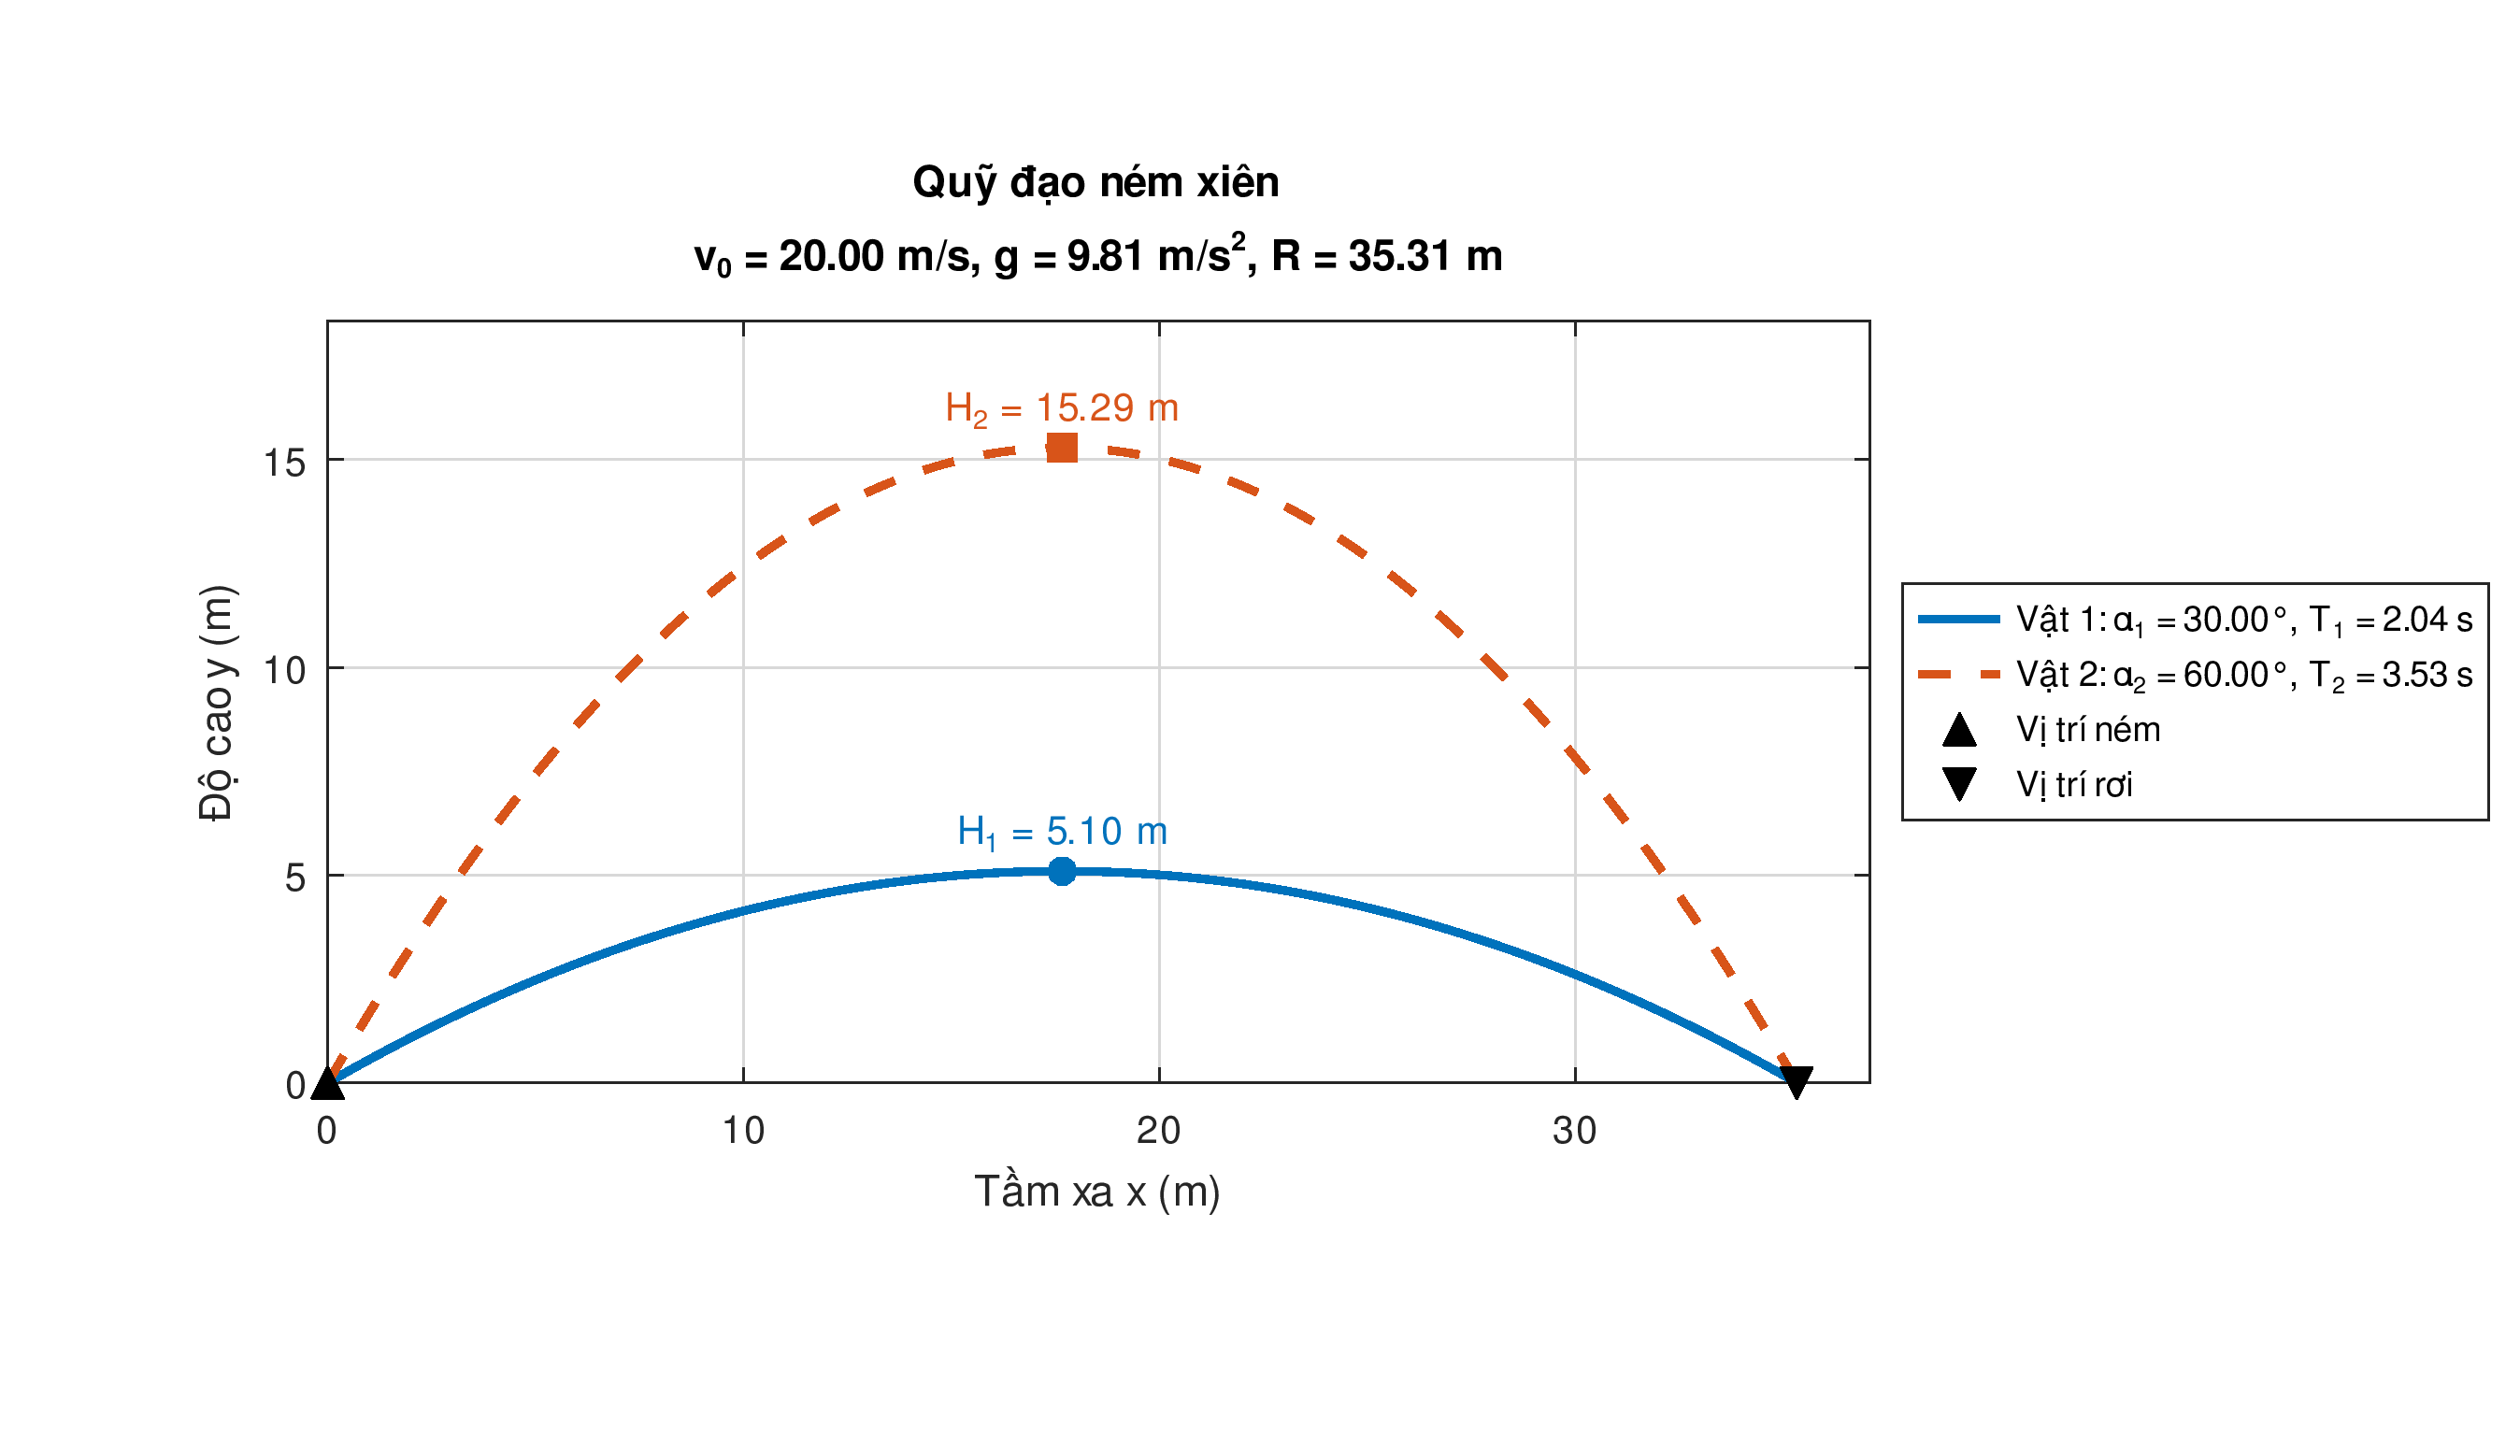
\includegraphics[width=0.9\textwidth]{quydao_v0_20_alpha1_30.png}
%   \caption{Quỹ đạo hai vật với $v_0 = 20$~m/s, $\alpha_1 = 30^\circ$}
%   \label{fig:quydao30}
% \end{figure}

\chapter{KIỂM THỬ CHƯƠNG TRÌNH VÀ XÁC MINH TÍNH ĐÚNG ĐẮN}
\section{Thiết kế các ca kiểm thử}
% TODO: dán nội dung từ Google Docs vào đây.

\section{Kết quả kiểm thử và đánh giá sai số}
% TODO: dán nội dung từ Google Docs vào đây.


\chapter{PHÂN TÍCH VÀ THẢO LUẬN KẾT QUẢ VẬT LÝ}
\section{So sánh đặc tính hai quỹ đạo có cùng tầm xa}
% TODO: dán nội dung từ Google Docs vào đây.

\section{Nhận xét về các đại lượng đặc trưng}
% TODO: dán nội dung từ Google Docs vào đây.


\chapter{KẾT LUẬN VÀ HƯỚNG PHÁT TRIỂN ĐỀ TÀI}
\section{Tóm tắt kết quả đạt được}
% TODO: dán nội dung từ Google Docs vào đây.

\section{Hạn chế và hướng mở rộng}
% TODO: dán nội dung từ Google Docs vào đây.



\unnumberedchapter{TÀI LIỆU THAM KHẢO}
\begin{enumerate}[label={[\arabic*]}]
  \item Nguyễn Thị Bé Bảy, Huỳnh Quang Linh, Trần Thị Ngọc Dung, \textit{Giáo trình Vật lý đại cương A1}, Trường Đại học Bách khoa -- ĐHQG TP.HCM.
  % TODO: bổ sung tài liệu tham khảo
\end{enumerate}


\unnumberedchapter{PHỤ LỤC}
\section*{Phụ lục A: Mã nguồn chương trình MATLAB}
\phantomsection\addcontentsline{toc}{section}{Phụ lục A: Mã nguồn chương trình MATLAB}
\subsection*{main.m}
\VerbatimInput{../src/main.m}

\subsection*{inputParameters.m}
\VerbatimInput{../src/inputParameters.m}

\subsection*{solveAngleSymbolic.m}
\VerbatimInput{../src/solveAngleSymbolic.m}

\subsection*{calculateProjectile.m}
\VerbatimInput{../src/calculateProjectile.m}

\subsection*{plotTrajectories.m}
\VerbatimInput{../src/plotTrajectories.m}

\subsection*{runTests.m}
\VerbatimInput{../src/runTests.m}


\end{document}
